\chapter{Introdução}

A introdução eu devo escrever por último, deve conter a importancia do projeto,
devo descrever o problema e a solução: "existe um problema e foi resolvido
assim". O final da introdução deve descrever a estrutura dos capitulos dando
uma pincelada rapida em cada um.

Este projeto consiste na implementação de um novo extrator para o egypt onde a
análise seja feita direto do código fonte sem necessidade de compilação. Com
isto será possível analisar projetos que não compilem mais, seja por falhas no
código ou por possuir dependencias não satisfeitas. Além disso, espera-se que
este novo extrator traga ainda mais duas vantagens: primeiro, o tempo
necessário para analisar um projeto cairá e segundo, as informações obtidas
serão mais precisas já que alguns dados importantes não se perderão como
acontece por exemplo com macros em projetos C/C++
\cite{SourceVersusObjectCodeExtraction} que se perdem com o extrator baseado em
GCC\sigla{GCC}{GNU C Compiler}.

\chapter{Conceitos}
\section{Arquitetura de Software}
\section{Atributos de Modularidade}
\subsection{Acoplamento}
\subsection{Coesão}

\chapter{Implementação do Extrator}

\section{egypt}

O egypt foi originalmente desenvolvido por Andreas
Gustafsson\footnote{http://www.gson.org/egypt} com o objetivo de gerar gráficos
de chamada entre funções de programas escritos em C, ele funciona lendo os
arquivos intermediários gerados pelo GCC e os
converte num gráfico de chamada no formato usado pelo
Graphviz\footnote{http://www.graphviz.org}, um programa para visualização de
gráficos.

O egypt é Software Livre e em Janeiro de 2009 começou a ser restruturado por
Antonio Terceiro o qual o tem mantido
em\footnote{http://github.com/terceiro/egypt}. As principais mudanças sofridas
pelo egypt deste então foram \cite{StructuralComplexityEvolution}:

\begin{itemize}
\item Detecção de uso de variáveis, para identificar que função usa qual
variável.
\item Opção para agrupar chamada e uso de variaveis por módulo, com isto é
possível ter uma visão de dependência entre módulos.
\item Refatoração do script egypt em um design orientado a objetos, para
permitir diferentes módulos de extração e relatório.
\item Geração de relatório de métricas, como coesão e acoplamento por exemplo.
\end{itemize}

Segue abaixo como ficou estruturado o egypt após a refatoração:

\begin{description}
\item[egypt] Script principal
\item[Egypt::Extractor] Extrator baseado nos arquivos intermediários do GCC
\item[Egypt::Metrics] Gera relatório de métricas com os dados do Egypt::Model
\item[Egypt::Model] Armazena os dados obtidos pelo extrator
\item[Egypt::Output::DOT] Gera saída no formato do Graphviz com os dados de Egypt::Model
\end{description}

\begin{figure}[h]
\center
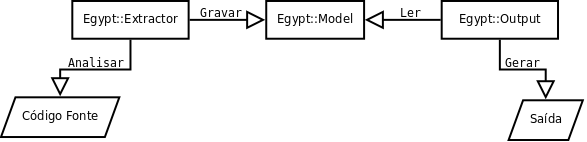
\includegraphics[scale=0.5]{imagens/egypt-fluxogram}
\caption{fluxograma de funcionamento do egypt}
\label{egypt-fluxogram}
\end{figure}

No fluxograma da figura~\ref{egypt-fluxogram} temos o seguinte: Egypt::Model é
alimentado com informações sobre declaração e uso de símbolos extraídos pelo
Egypt::Extractor e o Egypt::Output lê as informações contidas nele e gera saída
no formato apropriado.

\section{Doxygen (e a sua API)}

Doxygen\footnote{http://www.doxygen.org} é um sistema de documentação para C++,
C, Java, Objective-C, Python, IDL, Fortran, VHDL, PHP e C\#. Com ele é possível
gerar documentação em HTML, RTF, PostScript, PDF, \LaTeX\ e man pages, ele
extrai a documentação existente no código fonte e também extrai informações de
hierarquia e colaboração entre os módulos do projeto. É baseado nesta
capacidade de extrair informações hierarquia e colaboração que o Doxygen foi
escolhido como base para implementação deste novo extrator para o egypt.

O Doxygen é Software Livre e está disponível sob a GPL\sigla{GPL}{GNU Public
License}v2 em
\footnote{https://doxygen.svn.sourceforge.net/svnroot/doxygen/trunk}, junto aos
fontes deste programa existe um pequeno exemplo chamado doxyapp, que foi usado
como base para este projeto já que ele implementa uma ferramenta para análise
de código fonte bem próximo as necessidades deste projeto.

Entre as inúmeras classes presentes na API\sigla{API}{Application Programming
Interface (ou Interface de Programação de Aplicativos)} do Doxygen é importante
destacar as seguintes:

\begin{description}
\item[Doxygen] Provê um namespace para varáveis e funções globais usadas pelo doxygen
\item[CodeOutputInterface] Interface de saída de trecho de código para os parsers
\item[MemberDef] Definição de um membro ou símbolo de classe
\item[FileDef] Definição de um arquivo
\end{description}

\section{Implementação do Extrator usando a API do Doxygen}

O Doxygen apesar de oferecer todos os recursos necessários para
analisar projetos C/C++ e extrair o uso de símbolos, como funções e variáveis,
que é o objetivo deste projeto, não possibilita que a saída gerada seja
customizada, apenas oferece opções específicas como PDF e HTML por exemplo. É
necessário então adaptar o Doxygen para gerar uma saída num formato
específico e apenas com as informações necessárias, para isto foi criado o
doxyparse, um parser capaz de analisar códigos C/C++ extraindo símbolos
com a identificação de onde são declarados e onde são utilizados.

Seguindo a interface CodeOutputInterface foi possível reaproveitar no doxyparse
todo o poder que o Doxygen fornece e gerar a saída da forma desejada. Na
figura~\ref{doxyparse-diagram} temos o diagrama desta implementação.

\begin{figure}[h]
\center
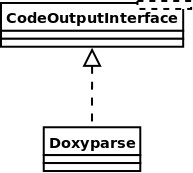
\includegraphics[scale=0.5]{imagens/doxyparse-diagram}
\caption{diagrama da hierarquia de classes do doxyparse}
\label{doxyparse-diagram}
\end{figure}

O doxyparse então reaproveita os recursos existentes no Doxygen para fazer a
análise de código e gerar uma saída que será lida pelo extrator a ser
implementado no egypt, ele redefine algums parâmetros de configuração
do Doxygen para obter o comportamento desejado, como: analisar diretórios
recursivamente, não gerar saida em Latex ou HTML, extrair tanta informação
quanto possível do código fonte, extrair informação de chamada e não gerar
mensagens de aviso.

O doxyparse faz então a análise dos fontes de um diretorio ou arquivo(s)
passados como parâmetro via linha de comando e extrai destes fontes os símbolos
encontrados. Após isto é gerada uma saída num formato específico que será lida
pelo extrator no egypt. Na figura~\ref{exemplo-saida-doxyparse} tem um exemplo
desta saída.

\begin{figure}[h]
\begin{Verbatim}[frame=single,fontsize=\relsize{-2},fontfamily=courier]
module module1.c
   function main in line 5
      uses function callback defined in module3.c
      uses function say_bye defined in module2.c
      uses function say_hello defined in module2.c
      uses variable variable defined in module3.c
\end{Verbatim}
\caption{exemplo de saída do doxyparse}
\label{exemplo-saida-doxyparse}
\end{figure}

Com a saída gerada pelo doxyparse o egypt precisa agora de um extrator que
entenda estes dados, extraia as informações sobre os símbolos e gere a saída no
formato do Graphviz que irá então gerar o gráfico de chamada entre os módulos.

O extrator atual do egypt, Egypt::Extractor, entende apenas arquivos
intermediários gerados pelo GCC e não é capaz de entender a saída da
figura~\ref{exemplo-saida-doxyparse}. Para isto foi necessário refatorar a
atual implementação do egypt e implementar um novo extrator. Na
figura~\ref{egypt-diagram-extractor} está o desenho desta nova estrutura.

\begin{figure}[h]
\center
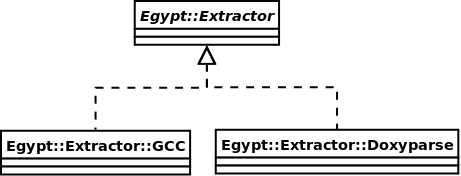
\includegraphics[scale=0.5]{imagens/egypt-diagram-extractor}
\caption{diagrama da hierarquia de classes do extrator do egypt}
\label{egypt-diagram-extractor}
\end{figure}

Abaixo uma breve descrição de cada classe presente na
figura~\ref{egypt-diagram-extractor}:

\begin{description}
\item[Egypt::Extractor] Interface padrão para os extratores.
\item[Egypt::Extractor::GCC] Extrator baseado nos arquivos intermediários do GCC.
\item[Egypt::Extractor::Doxyparse] Novo extrator baseado na saída do doxyparse
\end{description}

Após a refatoração demonstrada na figura~\ref{egypt-diagram-extractor} o egypt
pode extrair informações usando 2 métodos diferentes, usando o
Egypt::Extractor::GCC que faz a extração baseada nos arquivos intermediários do
GCC ou usando o Egypt::Extractor::Doxyparse que faz a análise utilizando o
doxyparse. Segue abaixo um exemplo de execução do egypt usando cada um dos
extratores:

\begin{Verbatim}[frame=single,fontsize=\relsize{-2},fontfamily=courier]
 $ egypt --extractor Doxyparse <arquivos>
 $ egypt --extractor GCC <arquivos>
\end{Verbatim}

\chapter{Avaliação}

Com o extrator pronto é necessário avaliar se as informações extraídas estão
corretas e se há diferenças em relação as informações extraídas pelo extrator
original do egypt baseado em GCC.

\section{Procedimento}

Em \cite{StructuralComplexityEvolution} foi feita uma análise do
ristretto\footnote{http://goodies.xfce.org/projects/applications/ristretto}, um
Software Livre escrito em C para visualização de imagens no ambiente Desktop
Xfce\footnote{http://www.xfce.org}, utilizando o extrator original do egypt, as
informações geradas por esta análise serão utilizadas aqui para comparação com
as informações extraídas pelo novo extrator baseado no doxyparse.

Além da comparação entre o extrator original e o novo extrator a saída
gerada pelo doxyparse, o parser baseado no Doxygen, será analisada em
comparação com o código fonte em busca de inconsistências em relação a
declaração e uso de símbolos encontrados.

\section{Resultados}

Com os dados extraidos pelo Egypt::Extractor::GCC e Egypt::Extractor::Doxyparse
foram gerados gráficos de dependencia entre os módulos do projeto ristretto das
versões 0.0.1 até a 0.0.21.


Para comparação entre os dois extratores foram selecionadas 3 versões do
ristretto para ser avaliado, nas figuras \ref{ristretto-0.0.1},
\ref{ristretto-0.0.11} e \ref{ristretto-0.0.21} estão gráficos de chamadas
entre módulos das versões 0.0.1, 0.0.11 e 0.0.21 do ristretto gerado pelo
Doxyparse e pelo GCC, algumas diferenças entre os gráficos gerados pelo GCC e
pelo Doxyparse foram notadas. 

\begin{figure}
\center
\subfigure[ristretto-0.0.1-doxyparse][Egypt::Extrator::Doxyparse]{
   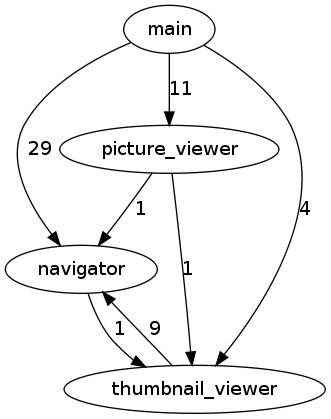
\includegraphics[scale=0.5]{imagens/ristretto-0_0_1-doxyparse}
}
\qquad
\subfigure[ristretto-0.0.1-gcc][Egypt::Extrator::GCC]{
   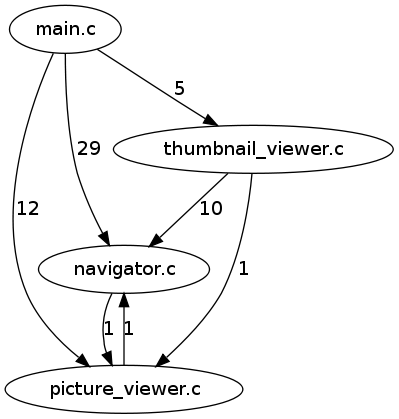
\includegraphics[scale=0.5]{imagens/ristretto-0_0_1-gcc}
}
\caption{gráfico de chamada entre módulos do {\bf Ristretto 0.0.1} gerado pelo Egypt}
\label{ristretto-0.0.1}
\end{figure}

Na figura~\ref{ristretto-0.0.1} nota-se uma diferença interessante entre as
informaçõe extraídas pelo GCC e o Doxyparse, há uma inversão entre os módulos
thumbnailer\_viewer e picture\_viewer. Enquanto o Doxyparse diz que o
picture\_viewer chama o thumbnailer\_viewer no GCC temos o contrário, após uma
verificação ao código fonte do ristretto 0.0.1 nota-se que nenhum dos 2 módulos
se referenciam, então tanto o extrator GCC quanto o extrator Doxyparse estão
dando informações incorretas.

Como o objetivo deste trabalho é o extrator Doxyparse faz-se necessário
procurar uma solução para este problema. O problema pode estar no doxyparse ou
no extrator Egypt::Extractor::Doxyparse.

Ao investigar o problema notou-se que o problema está no extrator não no
doxyparse em si. O egypt armazena as informações usando como chave, ou seja,
como identificador único, o nome do símbolo em questão mas alguns módulos
possuem símbolos com o mesmo nome, isto faz com que o egypt confunda o uso e
chamada desses símbolos.

A solução adotada para este problema foi armazenar o nome do símbolo junto ao
nome do módulo onde o símbolo está definido, por exemplo ao invés de guardar
apenas parent\_class guarda-se main::parent\_class.  Na figura
\ref{ristretto-0.0.1-doxyparse-2} na página
\pageref{ristretto-0.0.1-doxyparse-2} temos o gráfico atualizado após esta
correcão.

\begin{figure}
\center
\subfigure[ristretto-0.0.11-doxyparse][Egypt::Extrator::Doxyparse]{
   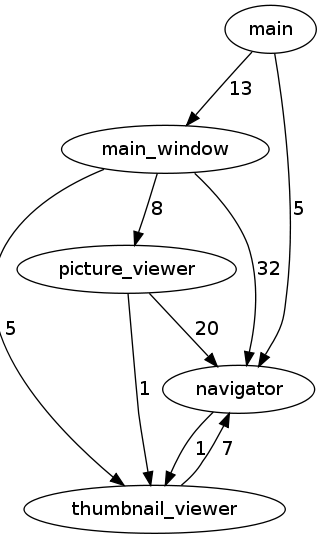
\includegraphics[scale=0.5]{imagens/ristretto-0_0_11-doxyparse}
}
\qquad
\subfigure[ristretto-0.0.11-gcc][Egypt::Extrator::GCC]{
   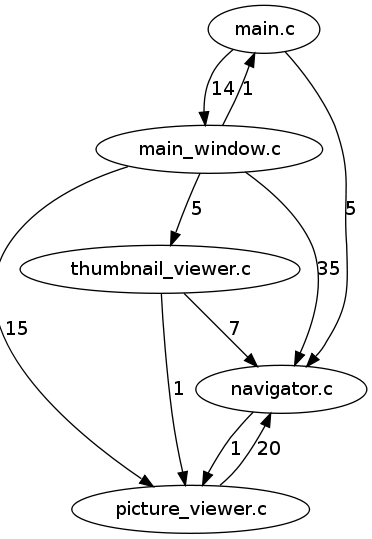
\includegraphics[scale=0.5]{imagens/ristretto-0_0_11-gcc}
}
\caption{gráfico de chamada entre módulos do {\bf Ristretto 0.0.11} gerado pelo Egypt}
\label{ristretto-0.0.11}
\end{figure}

O mesmo ocorre nas figuras \ref{ristretto-0.0.11} e \ref{ristretto-0.0.21}, mas
nestas outras ainda temos mais observações, por exemplo na
figura~\ref{ristretto-0.0.11} o GCC diz que o módulo main\_window chama main,
já no Doxyparse não há esta chamada. E de fato, analisando o código fonte do ristretto 0.0.11 não foi encontrado nenhuma chamada de main\_window para main. Este problema foi corrigido pela mesma correção feita no egypt para corrigir o problema encontrado na versao 0.1.1 do ristretto, na página \pageref{ristretto-0.0.11-doxyparse-2} está a figura~\ref{ristretto-0.0.11-doxyparse-2} contendo o gráfico atualizado.

\begin{figure}
\center
\subfigure[ristretto-0.0.21-doxyparse][Egypt::Extrator::Doxyparse]{
   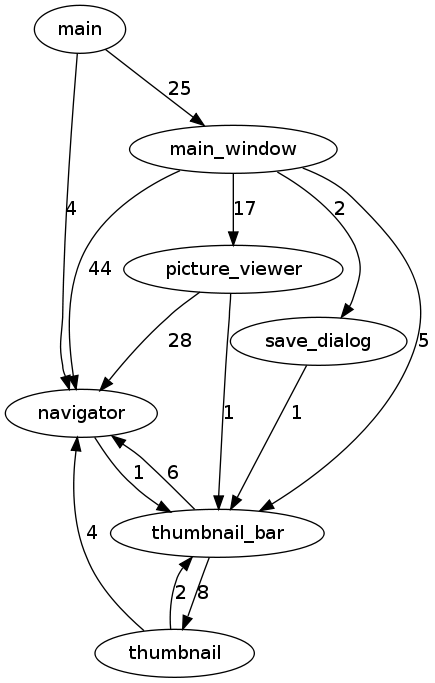
\includegraphics[scale=0.5]{imagens/ristretto-0_0_21-doxyparse}
}
\qquad
\subfigure[ristretto-0.0.21-gcc][Egypt::Extrator::GCC]{
   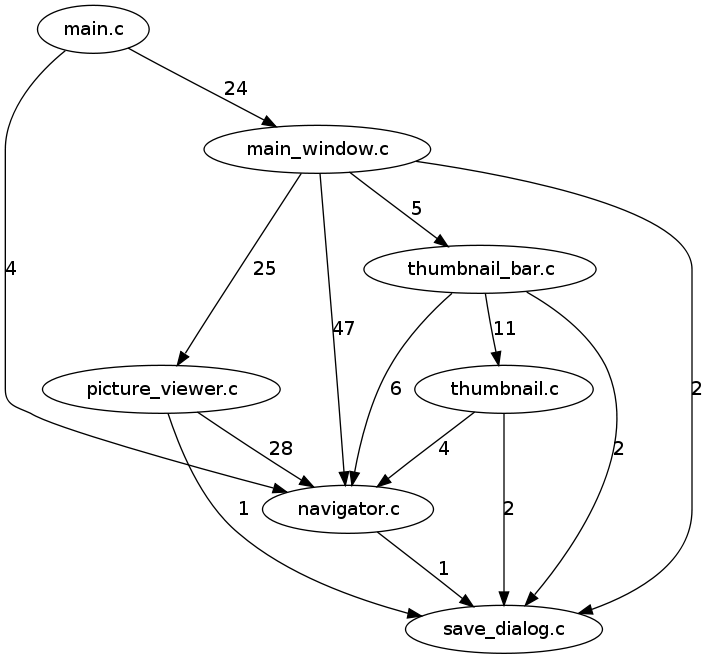
\includegraphics[scale=0.5]{imagens/ristretto-0_0_21-gcc}
}
\caption{gráfico de chamada entre módulos do {\bf Ristretto 0.0.21} gerado pelo Egypt}
\label{ristretto-0.0.21}
\end{figure}

Na figura~\ref{ristretto-0.0.21} temos ainda outra importante, o GCC nos diz
que o módulo save\_dialog é chamado por vários módulos: main\_window,
thumbnail, navigator, picture\_viewer e thumbnail\_bar sendo que no código
fonte do ristretto 0.0.21 não há indícios de que todos esses módulos chamem o
módulo save\_dialog, com excessão do main\_window que realmente chama
save\_dialog. Já o Doxyparse dá uma informação mais real onde apenas
main\_window chama save\_dialog, mas o Doxyparse dá uma informação controversa
onde o save\_dialog chama thumbnail\_bar e isto não foi confirmado analisando o
código fonte do projeto. Mas este problema foi causado pelo mesmo problema já
corrigido no egypt para o grafico do ristretto 0.0.1 e 0.0.11. O gráfico
corrigido está na figura~\ref{ristretto-0.0.21-doxyparse-2}
\ref{ristretto-0.0.21-doxyparse-2}

Além desta correção no Doxyparse foi necessário corrigir o doxyparse
que nestes casos confunde o uso do simbolo parent\_class que é uma variavei estática definida
por todos os módulos, mas o Doxygen registra este símbolo relacionado ao
primeiro módulo que ele analisa, e nos demais módulos que fazem uso dele o
Doxygen acha que o módulo está usando o simbolo definido no primeiro modulo
analisado. Isto foi solucionado ignorando as chamadas aos simbolos estaticos
fora do módulo sendo analisado, ou seja, só se considera chamada a símbolos
estaticos se eles estiverem no módulo que o simbolo foi encontrado.

\begin{figure}
\center
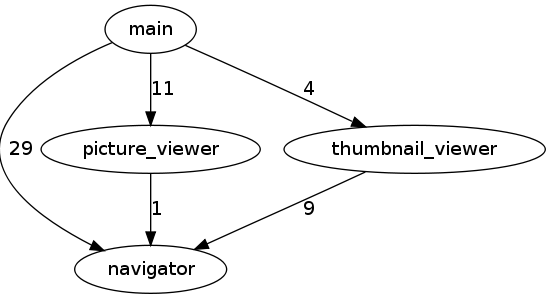
\includegraphics[scale=0.5]{imagens/ristretto-0_0_1-doxyparse-2}
\caption{gráfico de chamada entre módulos do {\bf Ristretto 0.0.1} gerado pelo Egypt::Extrator::Doxyparse atualizado}
\label{ristretto-0.0.1-doxyparse-2}
\end{figure}

\begin{figure}
\center
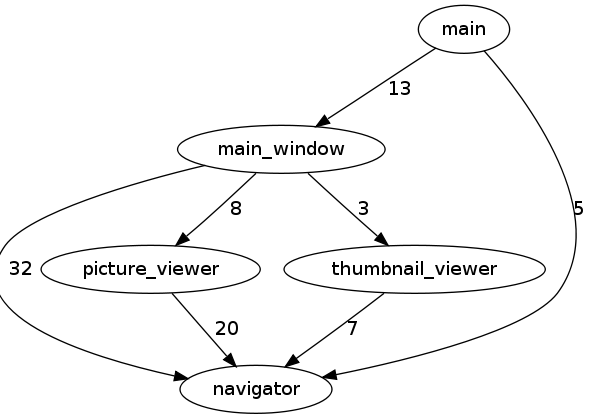
\includegraphics[scale=0.5]{imagens/ristretto-0_0_11-doxyparse-2}
\caption{gráfico de chamada entre módulos do {\bf Ristretto 0.0.11} gerado pelo Egypt::Extrator::Doxyparse atualizado}
\label{ristretto-0.0.11-doxyparse-2}
\end{figure}

\begin{figure}
\center
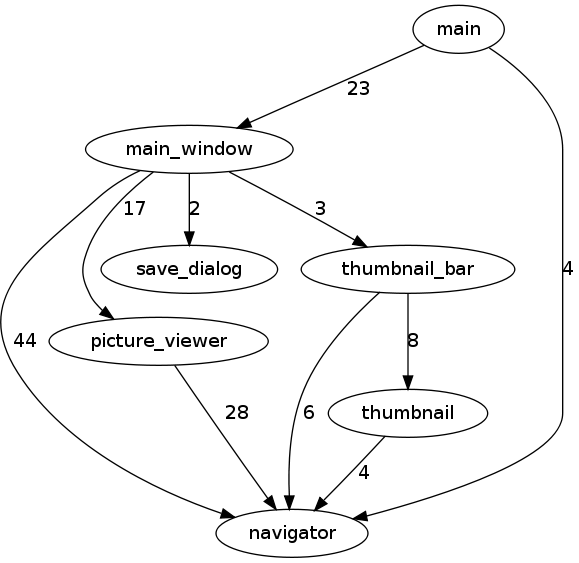
\includegraphics[scale=0.5]{imagens/ristretto-0_0_21-doxyparse-2}
\caption{gráfico de chamada entre módulos do {\bf Ristretto 0.0.21} gerado pelo Egypt::Extrator::Doxyparse atualizado}
\label{ristretto-0.0.21-doxyparse-2}
\end{figure}

\section{Discussão}

\chapter{Conclusão}

... Os resultados obtidos foram satisfatórios e atingiram o objetivo inicial que
foi possibilitar estração de dados sem necessidade de compilar o software em
questão, c ...

A conclusão eu devo escrever por último, deve conter algo assim: "Este trabalho
tinha objetivo tal e atingiu tal objetivo". Deve ter referencia de como foi
feito e se os resultados foram bons, medios, satisfatorios, ruins, etc. E ao
final deve ter trabalhos futuros que eu tenha interesse ou não de fazer.

Trabalhos futuros: verificar Natural Docs, semelhando ao Doxygen implementado
em Perl e suporta outras linguagens.
